\chapter{Gale Transformations and Diagrams}

A Gale transformation is a method of encoding the set of all of the affine dependencies of a \(d\)-dimensional set of points with cardinality \(n\ge d+1\) into a space of dimension \(n-d-1\).  This is exceptionally useful if \(n\) is not much larger than \(d\).  Usually this process is only applied to the vertex set of a polytope.

\section{Definition of Gale Transformation}

Let \(P\) be a \(d\)-polytope in \(\R d\) with \(\vrt P=V=\seta{\ve v_1,\ve v_2\dc \ve v_n}\) and consider the set of affine dependencies of \(V\), that is,
    \[
        \dep V
            =   \setb{(\la_1,\la_2\dc\la_n)\in\R n}{\sum_{i\in\brac n}\la_i\ve v_i=0\text{ and }\sum_{i\in\brac n}\la_i=0}.
    \]
Note that \(\dep V\) is an \((n-d-1)\)-dimensional vector space.  Let \(\seta{\ve a_1,\ve a_2\dc \ve a_{n-d-1}}\) be a basis of \(\dep V\), and write \(\ve a_i=(\alpha_{i,1},\alpha_{i,2}\dc \alpha_{i,n})\) for \(i\in\brac{n-d-1}\).  Now, let \(A\) be the \((n-d-1)\times n\) matrix whose \(i\)th row is \(\ve a_i\) for \(i\in\brac{n-d-1}\), and let \(\ol{\ve v}_j\) be the \(j\)th column of \(A\) for \(j\in\brac n\), that is,
    \[
        A
            =
                \begin{bmatrix}
                    \ve a_1\\ \ve a_2\\ \vdots\\ \ve a_{n-d-1}
                \end{bmatrix}
            =
                \begin{bmatrix}
                    \ol{\ve v}_1 & \ol{\ve v}_2 & \cdots & \ol{\ve v}_n
                \end{bmatrix}.
    \]
Then the (multi)set \(\ol V=\seta{\ol{\ve v}_1, \ol{\ve v}_2\dc \ol{\ve v}_n}\sbset\R{n-d-1}\) is a \dfn{Gale transformation} of \(V\) with \(\ol{\ve v}_i\) corresponding to \(\ve v_i\).  Define as well, for a subset \(X\sbset V\) the (multi)set \(\ol X=\setb{\ol{\ve v}\in\ol V}{\ve v\in X}\).

Note that there is not a unique Gale transformation for a given vertex set since a choice of basis was necessary.  This does nothing to detract from the usefulness of the construction.  Also, note that the definition did not require that the points \(\ve v_1,\ve v_2\dc\ve v_n\) be the vertex set of a polytope.  It was only necessary that \(\dim\aff V=d\).  Thus Gale diagrams can be defined for point sets satisfying this condition.

    \subsection{Computing a Gale Transformation}\label{SSec:ComputingGD}
    One method for actually computing a Gale transformation is as follows:

    Let \(P\) be a \(d\)-polytope in \(\R d\) with \(\vrt P=\seta{\ve v_1,\ve v_2\dc \ve v_n}\) ordered such that \(\ve v_1\dc \ve v_{d+1}\) are affinely independent.  Then
        \[
            \rref
            \begin{bmatrix}
                1       &1          &\cdots &1      \\
                \ve v_1 &\ve v_2    &\cdots &\ve v_n
            \end{bmatrix}
                =
                    \left[
                        \begin{array}{@{}c|c@{}}
                            I_{d+1} & N
                        \end{array}
                    \right]
        \]
    where \(N\) is some \((d+1)\times(n-d-1)\) matrix.  Setting
        \[
            \left[
                \begin{array}{@{}c|c@{}}
                    -N^{\text{T}}   &   I_{n-d-1}
                \end{array}
            \right]
                =
                    \begin{bmatrix}
                        \ol{\ve v}_1 &\ol{\ve v}_2    &\cdots &\ol{\ve v}_n
                    \end{bmatrix},
        \]
    yields a Gale transformation of \(\vrt P\), that is, the ordered (multi)set \(\seta{\ol{\ve v}_1, \ol{\ve v}_2\dc\ol{\ve v}_n}\).


\section{A Preliminary Result}\label{Sec:ConvAff}
    The following theorem will be crucial in the proof of Theorem \ref{Thm:CofaceIFF}, which provides the answer to the question, "Why should I care about Gale transformations?".  The proof closely follows that in \cite{Thomas}.
    \begin{Theorem}\label{Thm:ConvAff}
        If \(P\) is a \(d\)-polytope with \(V=\vrt(P)=\seta{\ve v_1,\ve v_2\dc\ve v_n}\sbset\R d\) and \(F\sbset V\), then \(\conv F\) is a face of \(P\) if and only if \(\conv(V\setminus F)\cap\aff(F)=\mt\).
    \end{Theorem}
    \begin{proof}
        Suppose, without loss of generality, \(F=\seta{\ve v_1,\ve v_2\dc\ve v_k}\) and \(\conv(F)\) is a face of \(P\).  Further, let \(H\) be a supporting hyperplane of \(F\) (so that \(\aff(F)\sbset H\)), say, \(H=\setb{\ve w}{\ip{\ve\xi}{\ve w}=t}\) with \(P\sbset H^+\).  Then the inclusions \(\ve v_j\in P\cap\left(\R d\setminus H\right)\) for all \(j>k\) imply that \(\ip{\ve\xi}{\ve v_j}>t\) for \(j>k\).  Let \(\ve x\in\conv(V\setminus F)\) with
            \begin{align*}
                \ve x&=\sum_{j\in\brac n\setminus\brac k}\alpha_j\ve v_j,
                    &   \sum_{j\in\brac n\setminus\brac k}\alpha_j&=1,
                    &   \alpha_j\ge0\text{ for all }j\in\brac n\setminus\brac k.
            \end{align*}
        Then
            \begin{align*}
                \ip{\ve\xi}{\ve x}
                    &=  \sum_{j\in\brac n\setminus\brac k}\alpha_j\ip{\ve\xi}{\ve v_j}
                    >   \sum_{j\in\brac n\setminus\brac k}\alpha_jt
                    =   t.
            \end{align*}
        Thus \(\ve x\in H^{(+)}=H^+\setminus H\).  Therefore, the inclusion \(\aff(F)\sbset H\) implies \(\conv(V\setminus F)\cap\aff(F)=\mt\).

        On the other hand, suppose \(\conv(V\setminus F)\cap\aff(F)=\mt\), and let \(\ve y_0\in\conv(V\setminus F)\).  Then
            \[
                \inf_{\ve x\in\aff(F)}\norm{\ve x-\ve y_0}
            \]
        is attained at \(\ve x_0\) when \(\aff\seta{\ve x_0,\ve y_0}\) is perpendicular to \(\aff(F)\).  Let \(H\) be the hyperplane through \(\ve x_0\) normal to \(\ve x_0-\ve y_0\).  Then
            \begin{enumerate}
                \item   \(\conv(V\setminus F)\cap H=\mt\) and
                \item   \(\aff(F)\sbset H\).
            \end{enumerate}
        Thus \(H\cap P=\conv F\) is a face of \(P\).
    \end{proof}

    \begin{Example}
        In Figure \ref{Fig:FivePts}, the set \(\conv\seta{\ve x_1,\ve x_4}\) is not a face of \(\conv\seta{\ve x_1,\ve x_2,\ve x_3,\ve x_4,\ve x_5}\) since \(\conv\seta{\ve x_2,\ve x_3,\ve x_5}\cap\aff\seta{\ve x_1,\ve x_4}\ne\mt\).
    \end{Example}
    \begin{center}
        \begin{figure}[h!bt]
            \includegraphics[page=20, width=.5\textwidth]{pictures.pdf}
            \caption{Example of Theorem \ref{Thm:ConvAff}.\label{Fig:FivePts}}
        \end{figure}
    \end{center}

\section{What is it good for?}
It turns out that it is more convenient to phrase the main theorem about Gale transformations in terms of the complement of a face of a polytope than the face itself. This section follows \cite{McMullenBook}.
\begin{Definition}
    Let \(P\) be a polytope with vertex set \(V\).  A subset \(X\) of the vertices is called a \dfn{coface} if \(\conv(V\setminus X)\) is a face of \(P\).  If \(\conv(V\setminus X)\) is a facet of \(P\), then \(X\) is called a \dfn{cofacet}.
\end{Definition}

\begin{Definition}
    Let \(X\) be a set of points in \(\R d\), and \(\ve x\) be any point of \(\R d\).  Then \(X\) is said to \dfn{capture} \(\ve x\) if \(\ve x\in\relint\conv X\), that is, \(\ve x\) is in the relative interior of the convex hull of \(X\).
\end{Definition}

The following theorem gives a characterization, in terms of a Gale transformation, of the cofaces of a polytope.  A proof of only one implication of the equivalence is given here.  The proof of the other implication can be found in \cite{GrunBook}, \cite{McMullenBook}, or \cite{Thomas}.\footnote{The proof of the implication given here is not explicitly given in any of these sources.}
\begin{Theorem}\label{Thm:CofaceIFF}
    Let \(P\) be a polytope, \(X\sbset V=\vrt P\), and \(\ol V\) be a Gale transformation of \(V\).  Then \(X\) is a coface of \(P\) if and only if either \(\ol X\) captures the origin or \(X=\mt\).
\end{Theorem}
\begin{proof}
    Let \(P\) be a \(d\)-polytope with \(V=\vrt P=\seta{\ve v_1,\ve v_2\dc\ve v_n}\sbset\R d\).

    If \(X=\mt\), then \(\vrt(P)\setminus X=\vrt P\), and \(P=\conv\vrt P\) is a face of \(P\).  Thus, suppose \(X\ne\mt\).

    Let \(I=\seta{i_1,i_2\dc i_r}\sbset\brac n\), \(J=\brac n\setminus I\), and \(X=\setb{\ve v_i}{i\in I}\).  Also, let
        \[
            \begin{bmatrix}
                \ol{\ve v}_1\\ \ol{\ve v}_2\\ \vdots\\ \ol{\ve v}_n
            \end{bmatrix}
                =
                \begin{bmatrix}
                    \ve w_1&\ve w_2&\cdots&\ve w_{n-d-1}
                \end{bmatrix}
        \]
    where the \(\ol{\ve v}_i\)'s are regarded as row vectors, and the \(\ve w_i\)'s are regarded as column vectors.

    Suppose \(\ve 0\notin\relint\conv\ol X\).  Then there is some hyperplane \(H=\setb{\ve y}{\ip{\ve\xi}{\ve y}=0}\sbset\R{n-d-1}\) with \(\ol{\ve v}_i\in H^+\) for each \(i\in I\) and there is some \(i_0\in I\) with \(\ve v_{i_0}\in H^{(+)}\).  Write \(\ve\xi=\Tr{\begin{bmatrix}\xi_1&\xi_2&\cdots&\xi_{n-d-1}\end{bmatrix}}\).

    For each \(i\in\brac n\), let \(\alpha_i=\ip{\ve\xi}{\ol{\ve v}_i}\) and \(S=\sum_{i\in I}\alpha_i\).  The inequalities \(\ip{\ve\xi}{\ol{\ve v}_i}\ge 0\) for \(i\in I\) and \(\ip{\ve\xi}{\ol{\ve v}_{i_0}}>0\) imply that \(S>0\).  Therefore, let \(\la_i=\alpha_i/S\), and \(\ve\la=\Tr{\begin{bmatrix}\la_1&\la_2&\cdots&\la_n\end{bmatrix}}\in\R n\).  Note that \(\ve\la\in\spn\seta{\ve w_1,\ve w_2\dc\ve w_{n-d-1}}=\dep(V)\); indeed:
        \begin{align*}
            \ve\la
                &=
                \begin{bmatrix}\la_1\\ \la_2\\ \vdots\\ \la_n\end{bmatrix}
                    =\frac1S
                    \begin{bmatrix}
                        \ip{\ve\xi}{\ol{\ve v}_1}\\ \ip{\ve\xi}{\ol{\ve v}_2}\\ \vdots\\ \ip{\ve\xi}{\ol{\ve v}_n}
                    \end{bmatrix}
                    =\frac1S
                    \begin{bmatrix}\ol{\ve v}_1\\ \ol{\ve v}_2\\ \vdots\\ \ol{\ve v}_n\end{bmatrix}
                    \begin{bmatrix}\xi_1\\ \xi_2\\ \vdots\\ \xi_{n-d-1}\end{bmatrix}
                    =\frac1S
                    \begin{bmatrix}\ve w_1&\ve w_2&\cdots&\ve w_{n-d-1}\end{bmatrix}
                    \begin{bmatrix}\xi_1\\ \xi_2\\ \vdots\\ \xi_{n-d-1}\end{bmatrix}\\
                &=
                \frac1S\sum_{i\in\brac{n-d-1}}\xi_i\ve w_i.
        \end{align*}
    Ergo, \(\sum_{i\in\brac n}\la_i\ve v_i=\ve 0\) and \(\sum_{i\in\brac n}\la_i=0\).  Set
        \[
            \ve z
                =
                \sum_{i\in I}\la_i\ve v_i
                =
                \sum_{i\in J}(-\la_i)\ve v_i
        \]
    and note that
        \[
            \sum_{i\in I}\la_i
                =
                \sum_{i\in I}\frac{\alpha_i}S
                =1
        \]
    and \(\la_i\ge0\) for \(i\in I\). Hence, \(\ve z\in\conv X\).  Further, \(\sum_{i\in J}(-\la_i)=1\), whence \(\ve z\in\aff(V\setminus X)\).  Thence, \(\aff(V\setminus X)\cap\conv(X)\ne\mt\).  Therefore, by Theorem \ref{Thm:ConvAff}, \(X\) is not a coface of \(P\).
\end{proof}

If \(P\) is a \(d\)-simplex in \(\R d\), then \(\card{\vrt P}=d+1\), and thus a Gale transformation of \(\vrt P\) is a subset of \(\R 0=\seta 0\).  Thus the only Gale transformation of a \(d\)-simplex is the multiset \(\seta{0,0\dc0}\) of \(d+1\) equal points.

\begin{Corollary}
    Let \(P\sbset\R d\) be a \(d\)-polytope with vertex set \(V=\vrt P\) of cardinality \(n>d+1\).  Also, let \(\ol V\) be a Gale transformation of \(P\), and \(H\) be a hyperplane in \(\R{n-d-1}\) with \(\ve 0\in H\).  Then
        \[
            \card{\ol V\cap H^{(+)}}\ge2.
        \]
    \begin{comment}
        If \(\ol V\) is a Gale transformation of the vertices \(V=\vrt P\) of a \(d\)-polytope \(P\sbset\R d\) with \(n\) vertices, and \(H\) is a hyperplane in \(\R{n-d-1}\) which contains \(\ve 0\), then either \(\card{\ol V\cap H^{(+)}}\ge2\), or \(P\) is a simplex.
    \end{comment}
\end{Corollary}
\begin{proof}
    Let \(P\) be a \(d\)-polytope in \(\R d\) that is not a simplex, and \(V=\vrt P=\seta{\ve v_1,\ve v_2\dc\ve v_n}\) be its vertex set.  Then each \(\ve v_i\) is a face of \(P\), so that \(V_i=V\setminus\seta{\ve v_i}\) is a coface of \(P\).  Hence, \(\ol V_i\) captures the origin.  If there were some hyperplane \(H\) containing \(\ve 0\) such that \(\ol V\cap H^{(+)}=\seta{\ol{\ve v}_i}\), then this could not happen.
\end{proof}

    If \(P\) is a polytope with vertex set \(V=\seta{\ve v_1,\ve v_2\dc\ve v_n}\), then a pair of vertices \(\ve v_i,\ve v_j\) is a \dfn{nonedge} of \(P\) if \(\conv\seta{\ve v_i,\ve v_j}\) is not a face of  \(P\).

\begin{Corollary}\label{Cor:Nonedge}
    If \(\ol V\) is a Gale transformation of the vertices \(V=\vrt P\) of a \(d\)-polytope \(P\sbset\R d\), then a pair of vertices \(\ve v_i,\ve v_j\) forms a nonedge of \(P\) if and only if there is some hyperplane \(H\) such that \(\ol V\cap H^{(+)}=\seta{\ol{\ve v}_i,\ol{\ve v}_j}\).
\end{Corollary}
\begin{proof}
    Let \(Q=\conv(\ol V\setminus\seta{\ol{\ve v}_i,\ol{\ve v}_j})\).

    If there is some hyperplane \(H\) containing the origin such that \(\ol V\cap H^{(+)}=\seta{\ol{\ve v}_i,\ol{\ve v}_j}\), then the set \(\ol V\setminus\seta{\ol{\ve v}_i,\ol{\ve v}_j}\) must have at least two points in \(H^{(-)}\), and none in \(H^{(+)}\) and therefore cannot capture the origin.

    The set \(\conv\seta{\ve v_i,\ve v_j}\) is a nonedge of \(P\) if and only if the set \(\ol V\setminus\seta{\ol{\ve v}_i,\ol{\ve v}_j}\) does not capture the origin.  Since \(Q\) is a convex set, it does not capture the origin if and only if there is some hyperplane \(H\) containing the origin with \(Q\sbset H^-\).  Notice that \(H^{(+)}\) must contain at least two points of \(\ol V\) since \(\ol V\) is a Gale transformation.  However, \(H^{(+)}\cap Q=\mt\), and therefore these two points must be \(\seta{\ol{\ve v}_i,\ol{\ve v}_j}\).
\end{proof}

The next theorem gives two conditions that, together, guarantee that a set of \(n\) points in \(\R{n-d-1}\) is a Gale transformation of the vertex set of some polytope.  The proof given closely follows that in \cite{McMullenBook}.

\begin{Theorem}\label{Thm:GaleTransOIf}
    Let \(X=\seta{\ve x_1, \ve x_2\dc\ve x_n}\) be a set of points in \(\R {k}\) such that
        \begin{enumerate}
            \item   \(\sum_{i\in\brac n}{\ve x}_i=\ve 0\) and
            \item   for all hyperplanes \(H\) containing \(\ve 0\) each open half-space contains at least two points of \(X\).
        \end{enumerate}
    Then \(X\) is a Gale transformation of the vertex set of some \(d\)-polytope.
\end{Theorem}
\begin{proof}
    Let \(X=\seta{\ve x_1, \ve x_2\dc\ve x_n}\) be a set of points in \(\R{k}\) satisfying the two conditions.  Also, let
        \[
            A
                =
                \begin{bmatrix}
                    \ve x_1 &\ve x_2 &\cdots &\ve x_n
                \end{bmatrix}
        \]
    be the matrix whose \(i\)th column is \(\ve x_i\).

    The second condition guarantees that \(X\) cannot be contained in any hyperplane containing the origin.  Thus \(\dim\spn X=k\), and therefore by the Rank-Nullity Theorem of Linear Algebra the dimension of the kernel of \(A\) is \(\dim\ker A=n-k\).

    Note that by the first condition \(\ve 1_n\in\ker A\), and hence the set \(\seta{\ve 1_n}\) can be extended to a basis of \(\ker A\), say \(\seta{\ve 1_n, \wt{\ve y}_1,\wt{\ve y}_2\dc\wt{\ve y}_{n-k-1}}\).  Let
        \[
            B
                =
                \begin{bmatrix}
                    \ve 1_n &\wt{\ve y}_1 &\wt{\ve y}_2 &\cdots &\wt{\ve y}_{n-k-1}
                \end{bmatrix}
                =
                \begin{bmatrix}
                    \wt{\ve x}_1\\ \wt{\ve x}_2\\ \vdots\\ \wt{\ve x}_n
                \end{bmatrix}.
        \]
    That is, the vectors \(\wt{\ve x}_i\) are the rows of the matrix \(B\) whose columns are \(\ve 1_n,\wt{\ve y}_1,\wt{\ve y}_2\dc\wt{\ve y}_{n-k-1}\).  Then, by definition, \(\seta{\ve x_1, \ve x_2\dc\ve x_n}\) is a Gale transformation of the set \(\wt X=\seta{\wt{\ve x}_1,\wt{\ve x}_2\dc\wt{\ve x}_n}\).  Now, by the second condition, and the previous theorem each \(\wt{\ve x}_i\) is a vertex of \(\conv\wt X\), and therefore \(\wt X\) is the vertex set of some polytope.
\end{proof}

\begin{Example}\label{Ex:GaleTrans}
    Let \(X=\seta{1,t,-t,-1}\) where \(t>0\), and note that \(X\) satisfies the hypotheses of Theorem \ref{Thm:GaleTransOIf}.  Following the proof, set
        \[
            B=
                \begin{bmatrix}
                    1   &-t &t\\
                    1   &1  &0\\
                    1   &0  &1\\
                    1   &0  &0
                \end{bmatrix}.
        \]
    Then \(X\) is a Gale transformation of the quadrilateral with vertices \(\begin{bmatrix}-t\\ t\end{bmatrix},\begin{bmatrix}1\\ 0\end{bmatrix},\begin{bmatrix}0\\ 1\end{bmatrix},\begin{bmatrix}0\\ 0\end{bmatrix}\).
\end{Example}

\section{Gale Diagrams}
If \(\ol V\) is a Gale transformation of the vertex set \(V\) of some polytope, and only the face lattice of the polytope is being considered, then the condition \(\sum_{\ol{\ve v}\in\ol V}\ol{\ve v}=\ve 0\) is superfluous.  The following definitions are made in light of this.

\begin{Definition}
    Suppose the multisets \(X=\seta{\ve x_1, \ve x_2\dc\ve x_n}\sbset\R k\) and \(Y=\seta{\ve y_1,\ve y_2\dc\ve y_n}\sbset\R k\) both capture \(\ve 0\).  Then \(X\) and \(Y\) are called \dfn{consubstantial} if for each \(J\sbset\brac n\) the sets \(\setb{\ve x_j}{j\in J}\) and \(\setb{\ve y_j}{j\in J}\) either both capture, or both do not capture \(\ve 0\).
\end{Definition}

Consubstantiality is an equivalence relation, and for a fixed polytope \(P\) the Gale transformations of \(\vrt P\) all lie in the same equivalence class.  However, if \(P\) is not a simplex, then there are multisets consubstantial to a Gale transformation of \(\vrt P\) that are not themselves Gale transformations.  For example, in \(\RR\), the multiset \(\seta{1,1,-1,-2}\) is consubstantial to the multiset \(\seta{1,1,-1,-1}\).  The former is not a Gale transformation of a polytope since \(1+1-1-2\ne0\).  However, the latter is (see Example \ref{Ex:GaleTrans}).

\begin{Definition}
    Suppose \(P\sbset\R d\) is a \(d\)-polytope with \(n\) vertices, and \(\ol V\) is a Gale transformation of \(V=\vrt P\).  If \(\Gamma\sbset\R{n-d-1}\) and \(\ol V\) are consubstantial, then \(\Gamma\) is called a \dfn{Gale diagram} of \(P\), and the equivalence class of all Gale diagrams of \(P\) is denoted \(\galed(P)\).
\end{Definition}

The following theorem shows the usefulness of Gale diagrams.

\begin{Theorem}
    Two polytopes \(P, Q\) are combinatorially equivalent if and only if \(\galed(P)=\galed(Q)\).
\end{Theorem}
\begin{proof}
    Suppose \(P\) and \(Q\) are combinatorially equivalent, that is, there is an isomorphism \(\varphi\) of face lattices \(\varphi\colon\fl P\rightarrow\fl Q\) (and therefore \(\card{\vrt P}=\card{\vrt Q}\)).  Write \(\vrt P=\seta{\ve p_1,\ve p_2\dc\ve p_n}\) and \(\vrt Q=\seta{\ve q_1,\ve q_2\dc\ve q_n}\) ordered such that \(\varphi(\ve p_i)=\ve q_i\) for each \(i\in\brac n\).

    The set \(\Gamma=\seta{\ve g_1,\ve g_2\dc\ve g_n}\in\galed(P)\) is a Gale diagram of \(P\) if and only if for each \(I\sbset\brac n\) such that \(\setb{\ve g_i}{i\in I}\) captures the \(\ve0\) the set \(\setb{\ve p_i}{i\in I}\) is a coface of \(P\).  This happens if and only if \(\setb{\ve q_i}{i\in I}\) is a coface of \(Q\) (via the isomorphism \(\varphi\)).  This is equivalent to  \(G\in\galed(Q)\). Thus \(\galed(Q)=\galed(P)\).

    On the other hand, suppose that \(\galed(P)=\galed(Q)\) (and therefore that \(\card{\vrt P}=\card{\vrt Q}\)).  Also, let \(G=\seta{\ve g_1,\ve g_2\dc\ve g_n}\in\galed(P)=\galed(Q)\), and order the sets  \(\vrt P=\seta{\ve p_1,\ve p_2\dc\ve p_n}\) and \(\vrt Q=\seta{\ve q_1,\ve q_2\dc\ve q_n}\) such that \(\ve g_i\) corresponds to both \(\ve p_i\) and \(\ve q_i\) for each \(i\in\brac n\).

    Define \(\vartheta\colon2^{\vrt P}\rightarrow2^{\vrt Q}\) (where \(2^X\) denotes the power set of the set \(X\)) by, for \(i\sbset\brac n\), \(\vartheta(\setb{\ve p_i}{i\in I})=\setb{\ve q_i}{i\in I}\).  Then \(\setb{\ve p_i}{i\in I}\) is a face of \(P\) if and only if \(\setb{\ve g_i}{i\in\brac n\setminus I}\) captures \(\ve0\).  This happens if and only if \(\vartheta(\setb{\ve p_i}{i\in I})=\setb{\ve q_i}{i\in I}\) is a face of \(Q\).  Hence \(\vartheta\) is an invertible map that sends faces of \(P\) to faces of \(Q\).  Furthermore, \(\setb{\ve p_j}{j\in J}\sbset\setb{\ve p_i}{i\in I}\) if and only if \(J\sbset I\) if and only if
        \[
            \vartheta(\setb{\ve p_j}{j\in J})
                =       \setb{\ve q_j}{j\in J}
                \sbset  \setb{\ve q_i}{i\in I}
                =       \vartheta(\setb{\ve p_i}{i\in I}),
        \]
    whence \(\vartheta\) is order preserving.  Thence, \(\vartheta\) induces an isomorphism \(\eta\colon\fl P\rightarrow\fl Q\).
\end{proof}

The following theorem follows immediately from Theorem \ref{Thm:GaleTransOIf} and can be found in \cite{McMullenBook}.  It is the condition that the program in Appendix \ref{Appendix:Program} uses to check whether or not a set of points is a Gale diagram of some polytope.

\begin{Theorem}
    Suppose \(n\ge0\) and \(d\ge-1\) are integers such that \(n\ge d+1\).  Then a set of points \(\Gamma=\seta{\ve g_1,\ve g_2\dc\ve g_n}\sbset\R{n-d-1}\) is a Gale diagram of some \(d\)-polytope \(P\) with \(\card{\vrt P}=n\) if and only if for each hyperplane \(H\sbset\R{n-d-1}\) with \(\ve 0\in H\) the cardinality \(\card{G\cap H^{(+)}}\ge 2\).
\end{Theorem}

In practice, one ``only'' needs to check the hyperplanes through the origin that are the span of \(n-d-2\) points in \(G\), that is, at most \(\binom{n}{n-d-2}=\binom{n}{d+2}\) distinct hyperplanes.  Further, since both orientations of a hyperplane need to be checked, after computing \(\card{G\cap H^{(+)}}\), one can immediately compute \(\card{G\cap H^{(-)}}\).


The following theorem gives a characterization of apices of pyramids and can be found in \cite{McMullenBook}.
\begin{Theorem}\label{Thm:GalePyr}
    If \(\Gamma\in\galed(P)\), then \(P\) is a pyramid with apex \(\ve x\) if and only if \(\ol{\ve x}=\ve 0\).
\end{Theorem}
\begin{proof}
    The point \(\ol{\ve x}=\ve 0\) if and only if \(\relint\conv\seta{\ol{\ve x}}=\seta{\ve0}\) if and only if \(\conv(\vrt(P)\setminus\seta{\ve x})\) is a face of \(P\).  Hence \(P\) is a pyramid with apex \(\ve x\).
\end{proof}

Suppose \(\seta{\ol{\ve x}_1,\ol{\ve x}_2\dc\ol{\ve x}_n}\) is a Gale transformation of a \(d\)-polytope \(P\sbset \R d\) with vertex set \(\seta{\ve x_1,\ve x_2\dc\ve x_n}\) and \(\seta{\alpha_1,\alpha_2\dc\alpha_n}\sbset\RR\) is a set of positive real numbers.  Then the (multi)set \(\seta{\alpha_1\ol{\ve x}_1,\alpha_2\ol{\ve x}_2\dc\alpha_n\ol{\ve x}_n}\) is a Gale diagram of \(P\).  Similarly, if \(\seta{\ve g_1,\ve g_2\dc\ve g_n}\) is a Gale diagram of \(P\), then there are positive real numbers \(\beta_1,\beta_2\dc\beta_n\) such that \(\sum_{i\in\brac n}\beta_i\ve g_i=\ve 0\).  Therefore, \(\seta{\beta_1\ve g_1,\beta_2\ve g_2\dc\beta_n\ve g_n}\in\galed(P)\) is a Gale transformation of \(P\).  Hence one can easily move between Gale transformations and Gale diagrams if necessary.

\section{Standard Gale Diagrams}
Gale diagrams (like most things) are easier to work with when they lie in a nice subset of the ambient space\footnote{Here, `nice' has the completely circular meaning of a subset that makes a Gale diagram easy to work with.}.  Points corresponding to apices of pyramids cannot be moved in a Gale diagram (Theorem \ref{Thm:GalePyr}), however each other point in a Gale diagram can be moved along the ray from the origin passing through that point (and possibly through a larger set), thus a natural construction is to performing the rescaling
    \[
        \ve g_i
            \longmapsto
            \begin{cases}
                \ve 0                   &\text{if }\ve g_i=\ve 0\\
                \ve g_i/\norm{\ve g_i}  &\text{if }\ve g_i\ne\ve 0
            \end{cases}
    \]
which places all points corresponding to non-apices on the unit sphere \(\Sp{n-d-2}\sbset\R{n-d-1}\).  A Gale diagram that is a subset of \(\Sp{n-d-2}\cup\seta{\ve 0}\) is called a \dfn{standard} Gale diagram.

\begin{comment}
    Standard Gale diagrams are useful aids in proving theorems like (\cite{McMullenBook} ):
\begin{Theorem}
    There are \(\floor{d^2/4}\) distinct combinatorial types of \(d\)-polytopes with \(d+2\) vertices, \(\floor{d/2}\) of which are simplicial.
\end{Theorem}
    \begin{proof}
        The following is only a proof of the first part of the theorem.

        Let \(n(d)\) be the number of combinatorial types of \(d\)-polytopes with \(d+2\) vertices.

        A \(d\)-dimensional polytope with \(d+2\) vertices has a \(1\)-dimensional Gale diagram, and is therefore completely characterized by two numbers; the number of points on each side of the origin.  The number of points at the origin is \(d+2\) minus the sum of these two numbers.  Thus \(n(d)\) can be determined by counting the number of unordered pairs \(\seta{a,b}\) with \(2\le a\le b\le\floor{d/2}\).  This number is \(\floor{d/2}\left\lceil d/2\right\rceil=\floor{d^2/4}\).
    \end{proof}

The proof of the first pat will be put off until section \ref{SSec:dPlusTwo}.   The proof of the second part of the theorem follows from the the fact that if \(\Gamma\) is a Gale diagram of a \(d\)-polytope \(P\) with \(n\) vertices, then \(P\) is a simplicial polytope if and only if for every hyperplane \(H\in\R{n-d-1}\) containing \(\ve 0\) the following holds:
    \[
        \ve 0
            \notin \relint\conv(\Gamma\cap H).
    \]
The proof of which can be found in \cite{McMullenBook}.
\end{comment}

\section{Examples}

\subsection{Crosspolytopes}
    Let \(\ve e_i\) be the \(i\)th unit basis vector in \(\R d\) and consider \(\xp d=\conv\seta{\pm\ve e_1,\pm\ve e_2\dc\pm\ve e_d}\), the standard \(d\)-crosspolytope.  Computing a Gale transformation of \(\xp d\) requires finding a basis for the kernel of the matrix
        \[
            \begin{bmatrix}
                1       &   1       &   \dotsb &   1&           1       &   1        &   1            &   \dotsb &   1          \\
                \ve e_1 &   \ve e_2 &   \dotsb &   \ve e_{d-1} &\ve e_d &   -\ve e_d &   -\ve e_{d-1} &   \dotsb &   -\ve e_1
            \end{bmatrix}.
        \]
    First, note that this is a \((d+1)\times(2d)\) matrix with rank \(d+1\).  Thus, the kernel has dimension \(d-1\).  The set \(\setb{\ve e_i+\ve e_{2d+1-i}-\ve e_1-\ve e_{2d}}{i\in\brac d\setminus\seta{1}}\) of \(d-1\) vectors in \(\R{2d}\) is linearly independent, and is a subset of the kernel.  Thus this set forms a basis.  Forming the matrix that has these vectors for its columns, and extracting the row vectors yields the Gale transformation \(\seta{-\ve 1,\ve e_1,\ve e_2\dc\ve e_{d-2},\ve e_{d-1},\ve e_{d-1},\ve e_{d-2}\dc\ve e_2,\ve e_1,-\ve 1}\sbset\R{d-1}\).  See Figure \ref{Fig:xp3Gale} for an illustration of the \(3\)-dimensional case.
    \begin{figure}[hbt]
        \centering
            \includegraphics[width=.7\textwidth, page=14]{pictures.pdf}
        \caption{The polytope $\xp 3$ and a Gale transformation of its vertices.\label{Fig:xp3Gale}}
    \end{figure}
    \begin{figure}[hbt]
        \centering
            \includegraphics[width=.7\textwidth, page=15]{pictures.pdf}
        \caption{A $3$-dimensional crosspolytope and a Gale transformation of its vertices.\label{Fig:x3Gale}}
    \end{figure}

    Thus a Gale diagram of the \(d\)-dimensional crosspolytope can be given by the vertices of a \((d-1)\)-simplex with the origin in its relative interior where each point occurs twice and corresponds to a pair of vertices that are not joined by an edge.  These are not all of the Gale diagrams of crosspolytopes; any doubled point can be split into two points as long as the two points are not moved ``too far'' apart \footnote{Here, ``too far'' has nothing to do with distance.  It is entirely possible that one point can be moved freely within an unbounded region if all other points are held fixed, e.g.{}, in Figure \ref{Fig:x3Gale} the point $\ol{\ve e_3}$ could be moved anywhere within the open third quadrant without changing the combinatorial type of the polytope.}  (compare Figures \ref{Fig:xp3Gale} and \ref{Fig:x3Gale}).

\subsection{Prisms over Simplices}
    A prism over a \(d\)-simplex is a \((d+1)\)-dimensional polytope with \(2d+2\) vertices.  It thus has a \(d\)-dimensional Gale diagram.

    Let \(P\) be the prism over a \(d\)-simplex with vertices
        \begin{align*}
            \begin{bmatrix} \ve e_1     \\ 1    \end{bmatrix},
            \begin{bmatrix} \ve e_2     \\ 1    \end{bmatrix},
            \dotsc
            \begin{bmatrix} \ve e_d     \\ 1    \end{bmatrix},
            \begin{bmatrix} -\ve 1      \\ 1    \end{bmatrix},
            \begin{bmatrix} -\ve 1      \\ -1   \end{bmatrix},
            \begin{bmatrix} \ve e_d     \\ -1   \end{bmatrix},
            \begin{bmatrix} \ve e_{d-1} \\ -1   \end{bmatrix},
            \dotsc
            \begin{bmatrix} \ve e_1     \\ -1   \end{bmatrix},
        \end{align*}
    where \(\ve e_i\) is the \(i\)th standard basis vector in \(\R d\).

    Then the vectors
        \begin{align*}
                \begin{bmatrix}
                    -\ve e_i     \\
                    1           \\
                    -1          \\
                    \ve e_i
                \end{bmatrix}
        \end{align*}
    form a basis for the kernel of the matrix
        \begin{align*}
            \begin{bmatrix}
                1           &   1           &   1           &   1           &   1           &
                1           &   1           &   1           &   1           &   1           \\
                \ve e_1     &   \ve e_2     &   \cdots      &   \ve e_d     &   -\ve1       &
                -\ve1       &   \ve e_d     &   \ve e_{d-1} &   \cdots      &   \ve e_1     \\
                1           &   1           &   1           &   1           &   1           &
                -1          &   -1          &   -1          &   -1          &   -1          \\
            \end{bmatrix}
        \end{align*}
    so that the set
        \begin{align*}
            \seta{
            -\ve e_1, -\ve e_2\dc \ve 1, -\ve 1,\ve e_d,\ve e_{d-1}\dc\ve e_1
            }\sbset\R d
        \end{align*}
    is a Gale transformation of \(P\).

    In general a Gale diagram of \(P\) is given by the vertices of a simplex with the origin in its relative interior, along with the negatives of these points.  The pairs of points that are antipodal are points of the polytope that correspond to the same point in the original simplex.

    \begin{figure}[hbt]
        \centering
            \includegraphics[width=.7\textwidth, page=29]{pictures.pdf}
        \caption{The polytope $\prism{\Delta_2}$ and a Gale transformation of its vertices.\label{Fig:TriPrismGale}}
    \end{figure}

\section{Oriented Matroids}

This section will focus mainly on oriented matroids that arise from point configurations in a Euclidean space.  Such oriented matroids are called \dfn{realizable}.  The definition of a general oriented matroid will be given in the penultimate subsection, though it is not necessary for the rest of the narrative.

This section will closely follow \cite{ZieglerBook} and \cite{OrientedMatBook}.
    \subsection{Sign Vectors and Orthogonality}
        If \(n\in\N\), then a \dfn{sign vector of length \(n\)} is an element of the set \(\seta{-,0,+}^n\).    If \(\ve v\in\R n\), then the \dfn{sign vector of \(\ve v\)}, denoted \(\sgn\ve v\), is the sign vector of length \(n\) with coordinates
            \begin{align*}
                (\sgn\ve v)_i
                    =       \begin{cases}
                                -   &\text{if } v_i<0\\
                                0   &\text{if } v_i=0\\
                                +   &\text{if } v_i>0.
                            \end{cases}
            \end{align*}
        Define, also, \(-\sgn\ve v\) by
            \begin{align*}
                (-\sgn\ve v)_i
                    =       \begin{cases}
                                +   &\text{if } v_i<0\\
                                0   &\text{if } v_i=0\\
                                -   &\text{if } v_i>0.
                            \end{cases}
            \end{align*}
        The sign vector with all coordinates \(0\) is denoted \(\ve 0\), that is, \(\ve 0=\sgn\ve 0\).  No confusion should arise from this slight abuse of notation.  If \(V\sbset\R n\), then set \(\sgn V=\setb{\sgn\ve v}{\ve v\in V}\).  The support of an \(n\)-dimensional sign vector \(\ve v\) is the set \(\supp\ve v=\setb{i\in\brac n}{\ve v_i\neq0}\).  If \(S\) is a set of sign vectors, then \(\supp S=\cup_{\ve s\in S}\supp\ve s\).  A sign vector \(\ve s\in S\) is said to be of \dfn{minimal support} if for each \(\ve t\in S\) the inclusion \(\supp\ve t\sbset\supp\ve s\) implies \(\supp\ve t=\supp\ve s\).

        \begin{Definition}
        If \(\ve s\) and \(\ve t\) are two sign vectors of length \(n\), then they are said to be \dfn{orthogonal} if either:
            \begin{enumerate}
                \item   for all \(i\in\brac n\) either \(s_i=0\), or \(t_i=0\); or
                \item   there is a pair \(i,j\in\brac n\) with \(s_i=t_i\ne0\) and \(s_j=-t_j\ne0\).
            \end{enumerate}
        \end{Definition}
        This definition of orthogonality is reasonable, since two sign vectors \(\ve s,\ve t\) of length \(n\) are orthogonal if and only if there are two vectors \(\ve v,\ve w\in\R n\) with \(\ve s=\sgn\ve v\) and \(\ve t=\sgn\ve w\) such that \(\ip{\ve v}{\ve w}=0\).

        The notation \(\ve s\perp\ve t\) signifies that \(\ve s\) is orthogonal to \(\ve t\).  Notice that \(\ve s\perp\ve s\) if and only if \(\ve s\) is the vector that is \(0\) in each coordinate.  Orthogonality is also a symmetric relationship, i.{}e.{}, \(\ve s\perp\ve t\) if and only if \(\ve t\perp\ve s\).  Orthogonality of sign vectors is not transitive, just as orthogonality of vectors in \(\R n\) is not transitive.

        If \(S\) is a set of sign vectors of length \(n\), then the \dfn{dual} of \(S\) is the set
            \[
                S^\perp
                    =   \setb{\ve t\in\seta{-,0,+}^n}{\ve t\perp\ve s\text{ for all }\ve s\in S}.
            \]
        Notice that \(\ve 0\in S^\perp\) so that \(S^\perp\ne\mt\).

    \subsection{Realizable Oriented Matroids}\label{SSec:Realizable}
        Let \(X=\seta{\ve x_1,\ve x_2\dc \ve x_n}\sbset\R d\), and suppose that \(\aff X=\R d\).  Denote by \([X]\) the matrix whose \(i\)th column is \(\ve x_i\).  Consider the set of affine dependencies of \(X\), that is:

        \[
            \dep X
                =   \setb{\ve\la=(\la_1,\la_2\dc\la_n)\in\R n}{[X]\ve\la=\ve0\text{ and }\sum_{i\in\brac n}\la_i=0}.
        \]
        The set of \dfn{vectors of \(X\)} is the set \(\mc V(X)=\sgn(\dep X)\) of sign vectors of the points in \(\dep X\).\footnote{The elements of \(X\) are themselves vectors in that they are elements of a vector space.  They are not, regrettably, \emph{the vectors of \(X\)}.  This terminology, however unfortunate it may be, is standard in the study of oriented matroids.}

        A sign vector \(\ve s\in\mc V(X)\) of minimal support is called a \dfn{circuit} of \(X\).  The set of all circuits of \(X\) is denoted
            \[
                \mc C(X)
                    =   \setb{\ve s\in\mc V(X)}{\ve s\text{ is of minimal support}}.
            \]
        The set of \dfn{covectors of \(X\)} is the set \(\mc V(X)^\perp\), and the set of \dfn{cocircuits} is the set of covectors of minimal support.
            \[
                \mc C(X)^\perp
                    =   \setb{\ve s\in\mc V(X)^\perp}{\ve s\text{ is of minimal support}}.
            \]

        Any one of the sets \(\mc V(X), \mc V(X)^\perp,\mc C(X),\mc C(X)^\perp\) can be used to define a realizable oriented matroid, in the same way that a topology on a set can be defined by either open or closed sets.  That is, any one of these sets can be obtained from each of the others.  For details, see \cite[section 6.3]{ZieglerBook}.
            \subsubsection{Geometric Interpretation of \protect$\mc V(X)\protect$}
                Every \(\ve\la\in\dep X\setminus\{\ve0\}\) corresponds to a point \(\wt{\ve\la}\) that lies in \(\conv X\) in the following way:

                Let \(\ve\la\in\dep(X)\setminus\{\ve0\}\).  Define the positive and negative parts of \(\ve\la\) to be the sets of coordinates such that \(\ve\la\) is positive or negative respectively:
                \begin{align*}
                    \Pos{\ve\la}
                        &=  \setb{i}{\la_i>0}&
                    \Neg{\ve\la}
                        &=  \setb{i}{\la_i<0}.
                \end{align*}

                Now define \(\la_+=\sum_{i\in\Pos{\ve\la}}\la_i\) and \(\la_-=\sum_{i\in\Neg{\ve\la}}\la_i\).  The equality \(\sum\la_i=0\) implies \(\la_+=-\la_-\); further, \(\ve\la\neq\ve0\) implies \(\la_+\neq0\).  Finally, the equality \([X]\ve\la=\ve0\) yields that
                \begin{align*}
                    \sum_{i\in P(\ve\la)}\frac{\la_i}{\la_+}\ve x_i
                        =   -\sum_{i\in N(\ve\la)}\frac{\la_i}{\la_+}\ve x_i.
                \end{align*}

                Call this point \(\wt{\ve\la}\).  The previous paragraph shows that
                \[
                    \wt{\ve\la}
                        \in     \conv\setb{\ve x_i}{i\in P(\ve\la)}
                                    \cap    \conv\setb{\ve x_i}{i\in N(\ve\la)}.
                \]
                Conversely each of the points in the above intersections corresponds to at least one affine dependence of \(X\).  Furthermore, every point in a particular intersection of the type above has the same sign vector.
            \subsubsection{Geometric Interpretation of \protect$\mc V^\perp(X)\protect$}
                Intuitively, a sign vector in \(\mc V^\perp(X)\) keeps track of which side of some hyperplane each point of \(X\) lies on (or if it lies on the hyperplane itself).

                To this end, let \(H=\setb{\ve x}{\ip{\ve\xi}{\ve x}=t}\) be some hyperplane in \(\R d\), and define the sign vector \(\ve s(H)\) as follows:
                    \begin{align*}
                        (\ve s(H))_i
                            =
                                \begin{cases}
                                    +   &\text{if } \ip{\ve\xi}{\ve x_i}>t\\
                                    0   &\text{if } \ip{\ve\xi}{\ve x_i}=t\\
                                    -   &\text{if } \ip{\ve\xi}{\ve x_i}<t.
                                \end{cases}
                    \end{align*}
                Then this sign vector encodes which side of \(H\) each point of \(X\) lies on.  Notice that
                    \begin{align*}
                        \ve s(H)=\sgn\left(\Tr{[X]}\ve\xi-t\ve1\right).
                    \end{align*}
                Therefore
                    \[
                        \mc V^\perp(X)
                            =
                                \setb{\sgn\left(\Tr{[X]}\ve\xi-t\ve1\right)}{\ve\xi\in\R d\text{ and }t\in\RR}.
                    \]
            \begin{Example}
            Let \(X=\seta{\ve x_1, \ve x_2, \ve x_3, \ve x_4, \ve x_5}\sbset\R 2\) where
                \begin{align*}
                    \ve x_1
                        &=  \begin{bmatrix}
                                -1\\ 1
                            \end{bmatrix},&
                    \ve x_2
                        &=  \begin{bmatrix}
                                -1\\ 0
                            \end{bmatrix},&
                    \ve x_3
                        &=  \begin{bmatrix}
                                1\\ 0
                            \end{bmatrix},&
                    \ve x_4
                        &=  \begin{bmatrix}
                                1\\ 2
                            \end{bmatrix},&
                    \ve x_5
                        &=  \begin{bmatrix}
                                0\\ 2
                            \end{bmatrix}
                \end{align*}
            \begin{comment}
            \begin{figure}[h!]
                \centering
                    \includegraphics[page=2, width=.3\textwidth]{pictures.pdf}
            \end{figure}
            \end{comment}
        and consider the affine dependence \(\ve\la=\Tr{(4,-1,-1,4,-6)}\).  In this case, \(P(\ve\la)=\seta{1,4}\), \(N(\ve\la)=\seta{2,3,5}\) and \(\la_+=8\).
        Hence
            \[
                \wt{\ve\la}
                    =   \frac{\la_1x_1+\la_4x_4}{\la_+}
                    =   \begin{bmatrix}
                            0\\ 3/2
                        \end{bmatrix}
            \]
        which is a point along the line segment from \(\ve x_1\) to \(\ve x_4\) as well as a point inside the triangle with vertices \(\ve x_2\), \(\ve x_3\), \(\ve x_5\).
            \begin{figure}[h!]
                \centering
                    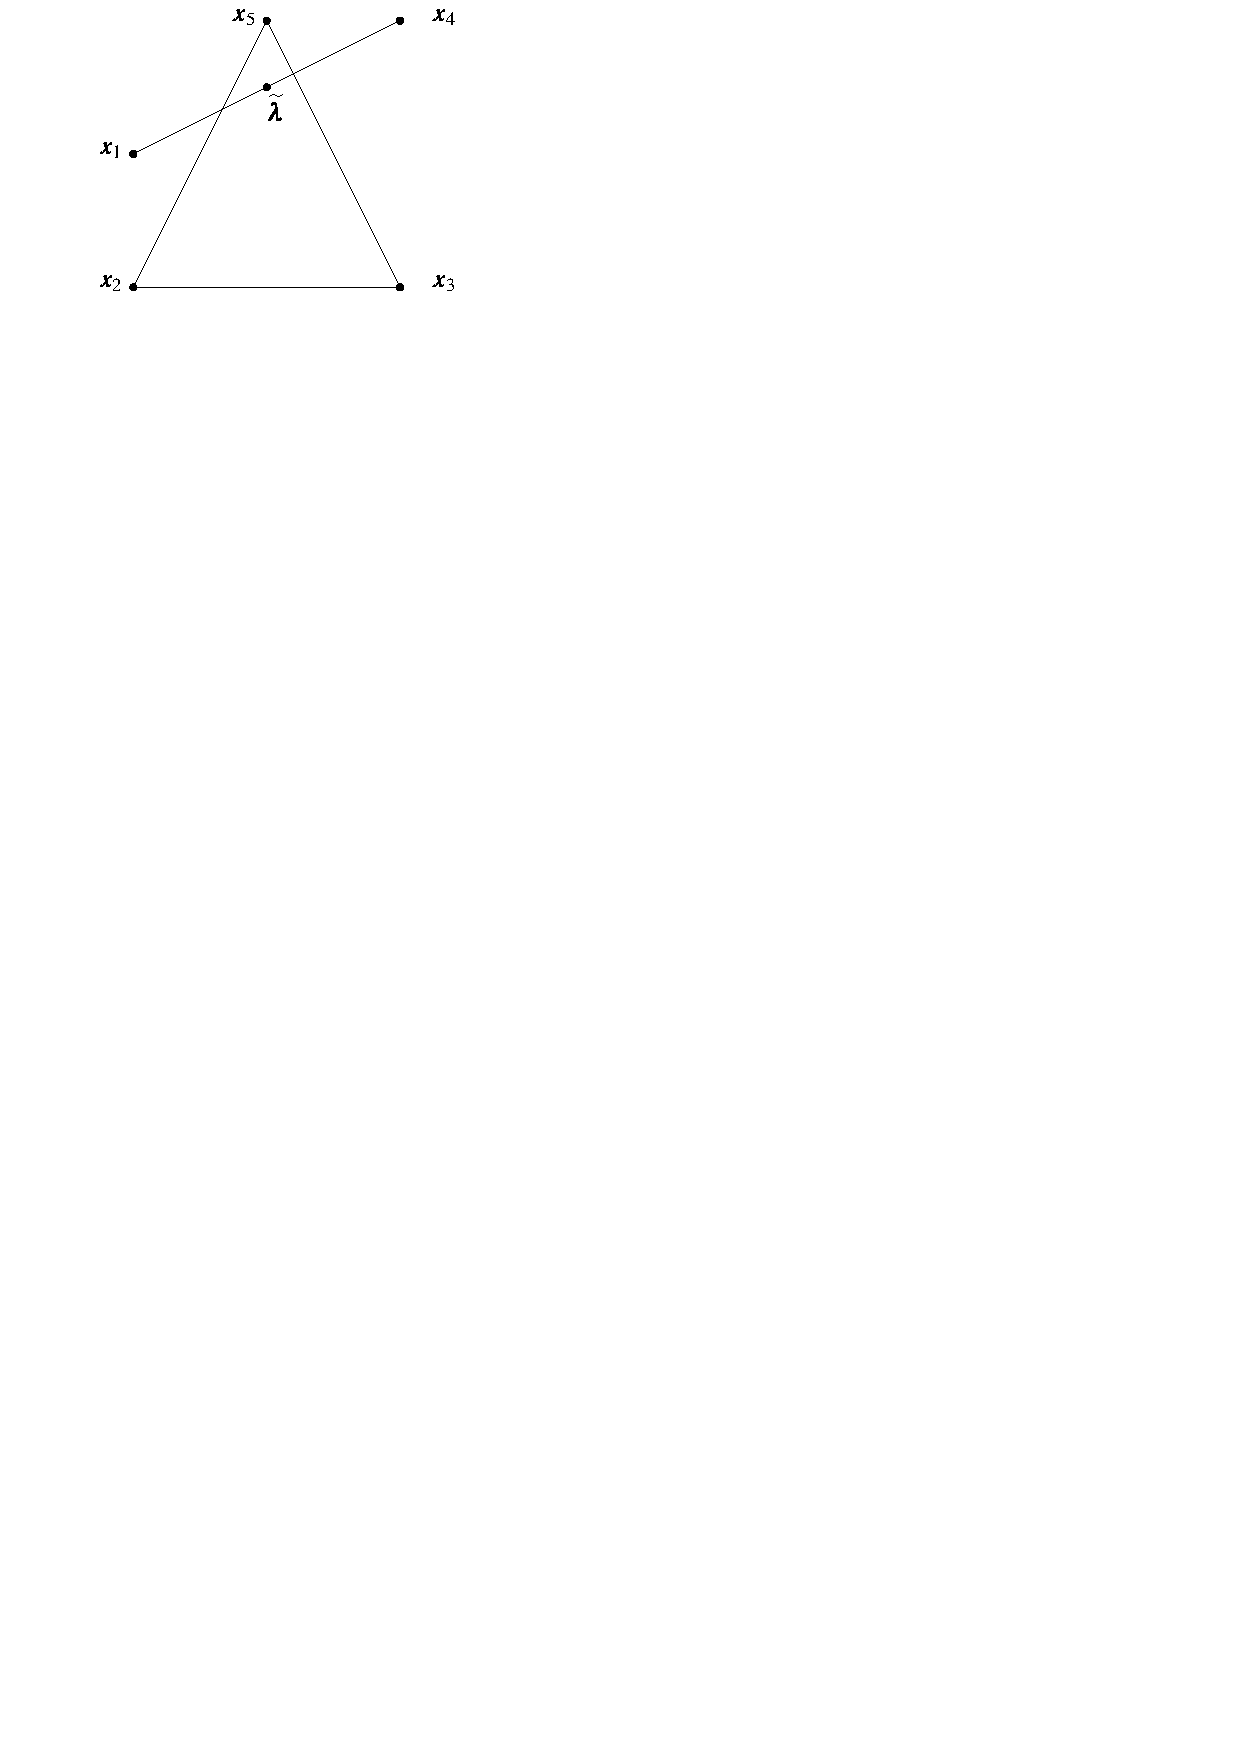
\includegraphics[page=1, width=.3\textwidth]{pictures.pdf}
            \end{figure}

        Further: \(\ve s=\sgn\ve\la=\usv+--+-\in\mc V(X)\); \(\card{\mc V(X)}=21\); and
            \begin{comment}
            \begin{align*}
                \mc V(X)
                    &=\left\{
                        \sv\ze+-+-, \sv+--+-,   \sv+-\ze+-, \snl
                        \sv+-+--,   \sv+-+-\ze, \sv+-+-+,   \snl
                        \sv+-+\ze-, \sv+-++-,   \sv+\ze-+-, \snl
                        \sv++-+-
                    \right\}
            \end{align*}
            \end{comment}
            \begin{align*}
                \mc C(X)
                    &=\left\{
                        \sv\ze+-+-,   \sv+-\ze+-,   \sv+-+-\ze, \snl
                        \sv+-+\ze-,   \sv+\ze-+-
                    \right\}.
            \end{align*}
            Note that \(\ve s\notin\mc C(X)\) since \(\ve t=\usv+-\ze+-\in\mc V(X)\) and \(\supp\ve t\varsubsetneq\supp\ve s\).  As for the dual sets, \(\card{\mc V^\perp(X)}=83\), and
            \begin{comment}
            \begin{align*}
                \mc V^*(X)
                    &=\left\{
                        \sv\ze\ze+++,  \sv\ze+---,    \sv\ze+\ze--,     \snl
                        \sv\ze++--,    \sv\ze++\ze-,  \sv\ze+++-,       \snl
                        \sv\ze+++\ze,  \sv\ze++++,    \sv+----,         \snl
                        \sv+---\ze,    \sv+---+,      \sv+--\ze+,       \snl
                        \sv+--++,      \sv+-\ze++,    \sv+-+++,         \snl
                        \sv+\ze---,    \sv+\ze--\ze,  \sv+\ze--+,       \snl
                        \sv+\ze-\ze+,  \sv+\ze-++,    \sv+\ze\ze++,     \snl
                        \sv+\ze+++,    \sv++---,      \sv++--\ze,       \snl
                        \sv++--+,      \sv++-\ze+,    \sv++-++,         \snl
                        \sv++\ze--,    \sv++\ze-\ze,  \sv++\ze-+,       \snl
                        \sv++\ze\ze+,  \sv++\ze++,    \sv+++--,         \snl
                        \sv+++-\ze,    \sv+++-+,      \sv+++\ze-,       \snl
                        \sv+++\ze\ze,  \sv+++\ze+,    \sv++++-,         \snl
                        \sv++++\ze,    \sv+++++
                    \right\}
            \end{align*}
            \end{comment}
            \begin{align*}
                \mc C^\perp(X)
                    &=\left\{
                        \sv\ze\ze+++,   \sv\ze+\ze--,   \sv\ze++\ze-,   \snl
                        \sv\ze+++\ze,   \sv+\ze--\ze,   \sv+\ze-\ze+,   \snl
                        \sv+\ze\ze++,   \sv++\ze-\ze,   \sv++\ze\ze+,   \snl
                        \sv+++\ze\ze
                    \right\}.
            \end{align*}
        \end{Example}

    \subsection{General Oriented Matroids}
        This section closely follows \cite[section 7.4]{ZieglerBook}.
        Before giving the definition of a general oriented matroid, three more definitions are needed for collections of sign vectors.
        \begin{Definition}  Let \(\ve s,\ve t,\ve u\) be sign vectors of length \(n\).
            \begin{enumerate}
                \item   The \dfn{composition} of  \(\ve s\) and \(\ve t\) is the sign vector \(\ve s\circ\ve t\) with coordinates
                        \begin{align*}
                            (\ve  s\circ\ve t)_i
                                =   \begin{cases}
                                        s_i     &   ,\text{ }s_i\ne0\\
                                        t_i     &   ,\text{ }s_i=0.
                                    \end{cases}
                        \end{align*}
                \item   The separation set of \(\ve s\) and \(\ve t\) is the set
                        \[
                            \sep{\ve s}{\ve t}
                                =   \setb{i\in\brac n}{s_i=-t_i\ne0}.
                        \]
                \item   If \(j\in\sep{\ve s}{\ve t}\), then \(\ve u\) \dfn{eliminates \(j\) between \(\ve s\) and \(\ve t\)} if \(u_j=0\) and for every \(i\notin\sep{\ve s}{\ve t}\), the equality \(u_i=(\ve s\circ\ve t)_i\) holds.
            \end{enumerate}
        \end{Definition}

        Notice that \(\sep{\ve s}{\ve t}=\sep{\ve t}{\ve s}\) and composition is not a commutative operation (Example \ref{Ex:OrientedOps}).  It is an associative operation since
            \begin{align*}
                (\ve s\circ(\ve t\circ\ve u))_i
                    =   ((\ve s\circ\ve t)\circ\ve u)_i
                    =   \begin{cases}
                            s_i     &,\text{ }s_i\ne0\\
                            t_i     &,\text{ }s_i=0\ne t_i\\
                            u_i     &,\text{ }s_i=0=t_i
                        \end{cases}.
            \end{align*}

        \begin{Example}\label{Ex:OrientedOps}
            Let \(\ve s=\usv+++0-\), and \(\ve t=\usv+-0++\).  Then
                \begin{itemize}
                    \item   \(\ve s\circ\ve t=\usv++++-\),
                    \item   \(\sep{\ve s}{\ve t}=\seta{2,5}\), and
                    \item   \(\ve u\) eliminates \(2\) between \(\ve s\) and \(\ve t\) if and only if \(\ve u\) is of the form \(\usv+0++\alpha\) for \(\alpha\in\seta{-,0,+}\).
                \end{itemize}

            On the other hand
                \begin{itemize}
                    \item   \(\ve t\circ\ve s=\usv+-+++\) and
                    \item   \(\ve u\) eliminates \(2\) between \(\ve t\) and \(\ve s\) if and only if \(\ve u\) is of the form \(=\usv+0++\beta\) for \(\beta\in\seta{-,0,+}\).
                \end{itemize}
        \end{Example}

        \begin{Definition}
            A set \(\mc V^\perp\sbset\seta{-,0,+}^n\) is the set of \dfn{covectors of an oriented matroid} if it satisfies the following:
                \begin{enumerate}
                    \item   \(\ve 0\in\mc V^\perp\);
                    \item   if \(\ve s\in\mc V^\perp\), then \(-\ve s\in\mc V^\perp\);
                    \item   if \(\ve s,\ve t\in\mc V^\perp\), then \(\ve s\circ\ve t\in\mc V^\perp\)
                    \item   if \(\ve s,\ve t\in\mc V^\perp\) and \(j\in\sep{\ve s}{\ve t}\), then there is some \(\ve u\in\mc V^\perp\) such that \(\ve u\) eliminates \(j\) between \(\ve s\) and \(\ve t\).
                \end{enumerate}
        \end{Definition}

        Covectors as described in section \ref{SSec:Realizable} satisfy the properties above, and therefore do form the set of covectors of an oriented matroid.


    \subsection{The Dual of an Oriented Matroid}
        For proofs of the results in this subsection, see either \cite{ZieglerBook} or \cite{OrientedMatBook}.

        Recall that the definition of orthogonality and dual were in terms of sign vectors.  Thus it makes sense to apply these operations to the covectors in a general oriented matroid.  In general, \((S^\perp)^\perp=S\).  Thus taking duals of a set leads to at most two distinct sets.  For \(\mc V^\perp\) the set of covectors of a general oriented matroid, define the \dfn{set of vectors} to be \(\mc V=(\mc V^\perp)^\perp\).  One can define circuits and cocircuits analogously.  Similar to the case of realizable oriented matroids, any of these four sets can be used to determine the others.

        A nontrivial result of oriented matroid theory is that the set of vectors of an oriented matroid is also the set of covectors of a different\footnote{As long as \(\mc V\ne\seta{\ve 0}\).  This follows since \(\mc V\cap\mc V^\perp=\seta{\ve 0}\).} oriented matroid.  This oriented matroid is called the \dfn{dual} of the original oriented matroid.

        In the case of a realizable oriented matroid (realized by the set of points \(V\)), the dual is also realizable, and is realized by a Gale diagram \(\Gamma\in\galed V\). 